% !TeX program = xelatex
% 面向数据发布前审查的电力数据隐性推断源定位方法（paper3）
\documentclass[UTF8,zihao=5,twoside,fontset=none]{ctexart}

\usepackage[paperwidth=210mm,paperheight=285mm,twoside=false,
            left=19.5mm,right=17.7mm,top=30mm,textheight=232mm,
            headheight=14pt,headsep=6mm,columnsep=7mm]{geometry}
\usepackage{fontspec}
\usepackage{xeCJK}
\usepackage{amsmath,amssymb,bm}
\usepackage{graphicx}
\usepackage{float}
\usepackage{booktabs,array,multirow,tabularx}
\usepackage{caption}
\usepackage{titlesec}
\usepackage{fancyhdr}
\usepackage{indentfirst}
\usepackage{enumitem}
\usepackage{tikz}
\usetikzlibrary{arrows.meta,positioning,shapes.geometric}
\usepackage[hidelinks]{hyperref}

\graphicspath{{figures/}}

\IfFontExistsTF{Songti SC}
  {\setCJKmainfont{Songti SC}}
  {\IfFontExistsTF{SimSun}
    {\setCJKmainfont{SimSun}}
    {\setCJKmainfont{FandolSong-Regular.otf}[BoldFont=FandolSong-Bold.otf,ItalicFont=FandolKai-Regular.otf]}}
\IfFontExistsTF{Heiti SC}
  {\setCJKsansfont{Heiti SC}}
  {\IfFontExistsTF{SimHei}
    {\setCJKsansfont{SimHei}}
    {\setCJKsansfont{FandolHei-Regular.otf}[BoldFont=FandolHei-Bold.otf]}}
\IfFontExistsTF{Times New Roman}{\setmainfont{Times New Roman}}%
  {\IfFontExistsTF{TeX Gyre Termes}{\setmainfont{TeX Gyre Termes}}{\setmainfont{Latin Modern Roman}}}

\zihao{5}
\setlength{\parindent}{2em}
\linespread{1.254}
\setlist{nosep,leftmargin=2em}
\setlength{\textfloatsep}{0.7em plus 0.2em minus 0.2em}
\setlength{\floatsep}{0.6em plus 0.2em minus 0.2em}
\setlength{\intextsep}{0.6em plus 0.2em minus 0.2em}
\renewcommand{\topfraction}{0.92}
\renewcommand{\bottomfraction}{0.85}
\renewcommand{\textfraction}{0.06}
\renewcommand{\floatpagefraction}{0.80}

\pagestyle{fancy}
\fancyhf{}
\fancyhead[LE]{\zihao{-5}第~\thepage~页}
\fancyhead[CE]{\zihao{-5}南方电网技术}
\fancyhead[RE]{\zihao{-5}第~XX~卷}
\fancyhead[LO]{\zihao{-5}\thepage}
\fancyhead[CO]{\zihao{-5}南方电网技术}
\fancyhead[RO]{\zihao{-5}第~XX~卷}
\renewcommand{\headrulewidth}{0.4pt}
\renewcommand{\footrulewidth}{0pt}

\titleformat{\section}{\sffamily\zihao{4}\bfseries}{\thesection}{0.6em}{}
\titleformat{\subsection}{\sffamily\zihao{5}\bfseries}{\thesubsection}{0.6em}{}
\titlespacing*{\section}{0pt}{0.8em}{0.4em}
\titlespacing*{\subsection}{0pt}{0.6em}{0.3em}

\captionsetup{font={small},labelfont=bf,labelsep=quad,justification=centering}
\renewcommand{\figurename}{图}
\renewcommand{\tablename}{表}
\renewcommand{\theequation}{\arabic{equation}}
\newcommand{\figbicaption}[2]{\caption{#1\\[-0.2em]\small Fig.\,\thefigure\ #2}}
\newcommand{\tabbicaption}[2]{\caption{#1\\[-0.2em]\small Tab.\,\thetable\ #2}}
\renewcommand{\refname}{参考文献}

\newcommand{\articleinfo}{文章编号：1674-0629(20XX)XX-XXXX-XX\quad 中图分类号：TM73\quad 文献标志码：A\\
DOI：10.13648/j.cnki.issn1674-0629.20XX.XX.XXX}

\begin{document}
\twocolumn[

\begin{center}
{\zihao{-5}\articleinfo}\par\vspace{1.0em}
{\sffamily\zihao{2}\bfseries 面向发布前审查的电力数据隐性推断源定位方法}\par\vspace{0.6em}
{\zihao{4}郑茂然$^{1}$，陶文伟$^{1}$，李家璐$^{1}$，雷傲宇$^{1}$，谭伟涛$^{2}$，王宏$^{2}$，杜浩存$^{2}$}\par\vspace{0.3em}
{\zihao{5}（1. 中国南方电力调度控制中心，广州 510663；2. 南方电网科学研究院有限责任公司，广州 510663）}\par\vspace{0.8em}
\end{center}

\noindent\textbf{摘要：}针对电网历史数据发布前审查中，多字段组合可能重构未发布运行状态的问题，提出一种前置关系剥离与输入稀疏门控相结合的推断源定位方法。将推断关系分为规则可解释关系和隐性统计关系：先依据数据定义、物理及会计关系剥离已知路径，再以归一化残差和反向消元排除高确定性替代路径；继而在剩余候选上引入分解式结构稀疏门控，并通过普通网络独立重训确认紧凑风险证据集。PJM 真实市场数据上，12 个目标平均使用 28.3\% 的字段取得 0.8512 的测试 $R^2$，全量字段为 0.8438；RTS-GMLC 算例中，18.9\% 的汇总发布字段可将具名设备状态平均重构到 0.9743。同预算下，所提方法在两个数据集上均取得最高平均精度，可为发布前字段组合审查提供依据。\par
\noindent\textbf{关键词：}电力数据发布；隐性推断；推断源定位；稀疏门控；数据安全\par\vspace{0.8em}

\begin{center}
{\bfseries\large Locating Implicit Inference Sources in Power Data for Pre-Release Review}\par\vspace{0.5em}
{ZHENG Maoran$^{1}$, TAO Wenwei$^{1}$, LI Jialu$^{1}$, LEI Aoyu$^{1}$, TAN Weitao$^{2}$, WANG Hong$^{2}$, DU Haocun$^{2}$}\par\vspace{0.3em}
{\small (1. CSG Power Dispatching Control Center, Guangzhou 510663, China; 2. Electric Power Research Institute of China Southern Power Grid Co., Ltd., Guangzhou 510663, China)}\par\vspace{0.5em}
\end{center}

\noindent\textbf{Abstract:} For pre-release review of historical power data, multiple release fields may jointly reconstruct non-released operational states. This paper proposes an inference-source localization method combining pre-localization relation stripping with input-wise sparse gating. Rule-explainable paths are first removed using data definitions and physical or accounting relations, followed by elimination of highly deterministic alternatives through normalized residuals and backward elimination. Factorized structured sparsity is then applied to the remaining input fields, and an ordinary network is independently retrained to verify a compact risk-evidence set. On PJM data, 28.3\% of the fields achieve an average test $R^2$ of 0.8512 over 12 targets, versus 0.8438 using all fields. On RTS-GMLC, 18.9\% of aggregate release fields reconstruct named device states to an average $R^2$ of 0.9743. The method achieves the highest mean accuracy on both datasets under equal feature budgets.\par
\noindent\textbf{Key words:} power-data release; implicit inference; inference-source localization; sparse gating; data security\par\vspace{0.8em}

\noindent{\zihao{6} 基金项目：国家科技重大专项课题资助项目（2026ZD0809803）；中国南方电网有限责任公司科技项目（ZDKJXM20240099）。\\
Foundation item: Supported by National Science and Technology Major Project (2026ZD0809803); Science and Technology Project of China Southern Power Grid Co., Ltd. (ZDKJXM20240099).}
\vspace{0.3em}
]

\section{引言}

电力系统运行、市场出清与调度控制数据由物理网络、运行规则和控制行为共同生成，字段之间存在显著的结构耦合。随着数据共享和市场信息披露范围扩大，发布审查不能只判断单个字段的密级：若干个可单独发布的汇总量、价格量或负荷量组合后，仍可能重构本次未发布的设备状态或运行细节。文献\cite{ref-liu-data-inference}将从低安全域数据恢复高安全域数据概括为信息物理融合系统中的数据推断威胁，并将状态估计、参数辨识和盲源分离纳入统一分析范式。本文进一步关注其中一个具体环节：\textbf{数据拥有方在批量发布历史数据之前，如何从拟发布字段中定位承载重构能力的字段集合}。

该场景的需求方是数据发布方的安全审查人员。审查人员掌握拟发布字段与受保护字段的内部历史联合样本，需要保守评估外部获得拟发布数据及部分历史配对样本后可能达到的重构能力。本文不讨论未来时刻预测，也不把模型精度提升作为最终目标；模型仅作为发布前的压力测试工具。审查输出应回答三个问题：目标是否可被重构，已知公式和业务规则能够解释哪些路径，剩余重构能力主要由哪些字段共同承载。

现有审查通常依赖字段名称、数据字典和人工规则。该方式能够发现电价分解、功率平衡和分量汇总等显式关系，却难以覆盖规则未记载的等价路径以及多字段共同形成的统计依赖。Pearson、Spearman、互信息和距离相关等指标计算简单，已用于电力负荷建模与数据清洗\cite{ref-lan-load,ref-jiao-pv,ref-deng-load,ref-szekely-dcorr,ref-reshef-mic}，但其描述的是单字段与目标的边际关系，不能判断该字段在联合推断中是否不可替代。Lasso、随机森林和 XGBoost 等方法可以给出重要性排序\cite{ref-tibshirani-lasso,ref-breiman-rf,ref-chen-xgboost}，但分别受到线性表达、冗余字段和事后解释偏差的影响；全量深度网络则只能说明“可以推到何种精度”，不能给出字段级审查结论。

因此，本文把发布前审查组织为两个相互衔接但边界明确的任务：先识别并剥离规则可解释的路径，再对剩余候选执行隐性推断源定位。这里的“两步剥离”只是进入定位模型之前的前置处理，不是第三类推断关系。全文仅区分两类风险：有明确规则或高确定性等价式可解释的第一类关系，以及剥离后仍可由联合统计依赖恢复的第二类隐性关系。

本文主要工作如下。

1）面向历史数据批量发布前审查，给出候选发布字段、受保护目标、攻击能力与审查输出的统一定义，将“能否推断”细化为显式关系清单、紧凑风险证据集和重构强度三个可计算量。

2）提出与推断源定位衔接的两步前置剥离方法。第一步依据数据定义和物理、会计关系建立规则库；第二步以归一化残差和反向消元搜索未记录的高确定性替代路径，避免后续网络被显式或近等价关系主导。

3）将分解式结构稀疏机制嵌入深度网络输入端，构造字段级稀疏门控定位模型，并以普通网络独立重训确认选中字段的联合推断能力。PJM 真实市场数据与 RTS-GMLC 设备状态算例分别用于算法验证和发布安全边界验证，并与 STG、LassoNet、XGBoost 等方法进行比较。

\section{发布前审查问题}

\subsection{场景与威胁模型}

设数据拥有方准备发布的字段为 $f_1,\ldots,f_n$，候选集合记为 $F$。内部保护目录将本次不发布的目标记为 $s_1,\ldots,s_m$，目标集合记为 $S$。拥有方在发布前可使用历史联合样本
\begin{equation}
\mathcal D=\{(\bm x_k,\bm y_k)\}_{k=1}^{N},\quad \bm x_k\in\mathbb R^n,\ \bm y_k\in\mathbb R^m
\end{equation}
进行审查。外部推断者被假定能够获得发布后的 $F$，并可能掌握同口径的历史配对样本或训练好的重构模型。审查方因此以容量充分的函数类 $\mathcal G$ 进行保守测试。对任意 $A\subseteq F$，定义目标 $s$ 关于 $A$ 的可推断性为
\begin{equation}
\rho(s\mid A)=\sup_{g\in\mathcal G}R^2\big(s,g(A)\big),
\end{equation}
其中 $R^2$ 在与训练过程独立的测试样本上计算：
\begin{equation}
R^2=1-\frac{\sum_{k=1}^{N_t}(y_k-\hat y_k)^2}{\sum_{k=1}^{N_t}(y_k-\bar y)^2}.
\end{equation}
式（2）描述的是审查能力上界，实验中以普通深度网络的测试 $R^2$ 近似。本文采用随机留出划分，对应已经形成的历史数据批次中，外部掌握部分配对样本并重构其余样本的场景；该结果不解释为未来时刻预测能力。

\subsection{两类推断关系}

若目标与候选字段之间的关系能够由数据字典、物理定律、市场规则或稳定等价式写成确定映射，则称为\textbf{规则可解释关系}。其形式包括守恒或会计恒等式、分量与汇总的组成关系以及口径确定的乘积或比值关系。此类关系能够形成可维护的规则清单，应在模型定位前单独处理。

若在规则路径剥离后不存在满足审查精度要求的显式映射，但目标仍能由候选字段的联合分布高精度恢复，则称为\textbf{隐性推断}。它来自潮流约束、机组组合、市场出清和调度策略长期共同作用形成的统计依赖，不能仅靠字段名称或两两相关性发现。承载该类联合重构能力的紧凑字段集合称为\textbf{隐性推断源}。

两类关系按规则的可复核性区分，而不是按模型种类区分。第一类输出规则及牵连字段；第二类输出紧凑证据集与可推断性。这样既能核对物理规律已经能够推断多少，又不会把显式公式造成的高精度误计为隐性推断能力。

\subsection{定位目标与输出边界}

设两步剥离后的候选池为 $\widetilde F$，理想的隐性推断源可表示为
\begin{equation}
A^*=\arg\min_{A\subseteq\widetilde F}|A|,
\quad \mathrm{s.t.}\quad
\rho(s\mid A)\geq \rho(s\mid\widetilde F)-\delta,
\end{equation}
其中 $\delta$ 为相对于全量候选模型允许的验证性能差。式（4）的作用不是寻找唯一因果解释，而是寻找一个尽可能小的\textbf{风险证据集}：只要少量拟发布字段即可接近全量字段的重构能力，就足以证明该发布组合存在集中风险。

电力数据常以不同口径重复携带同一信息，因而满足式（4）的集合可能不唯一。本文定位结果不能直接解释为“删除 $A^*$ 后风险必然消失”，也不把未选中字段称为无用字段。任何降精度、延迟或聚合方案实施后，都应在新候选池上重新执行完整审查。

\section{隐性推断源定位方法}

\subsection{总体流程}

方法如图~\ref{fig:flow} 所示。对每个受保护目标，先执行规则库剥离和高确定性路径逐层剥离，分别记录第一类关系清单并生成候选池 $\widetilde F$；随后训练字段级分解式稀疏门控网络，读取非零门控形成候选证据集；最后用不含门控的普通网络独立重训，输出字段占比与测试 $R^2$。因此，两步剥离发生在推断源定位之前，门控网络仅处理第二类隐性关系。

\begin{figure}[!tbp]
\centering
\begin{tikzpicture}[node distance=2.8mm,
  box/.style={draw,rounded corners=1pt,align=center,inner sep=2.2pt,
              font=\zihao{-5},text width=0.67\columnwidth,minimum height=6.3mm},
  tag/.style={font=\zihao{6},align=center,text=black!70},
  ar/.style={-{Latex[length=1.5mm]},thick}]
\node[box] (a) {输入：拟发布字段 $F$、受保护目标 $s$、内部历史样本};
\node[box,below=of a,fill=black!4] (b) {前置剥离 I：数据定义、物理及会计规则库};
\node[box,below=of b,fill=black!4] (c) {前置剥离 II：高确定性替代路径逐层搜索};
\node[box,below=of c] (d) {隐性关系候选池 $\widetilde F$};
\node[box,below=of d,fill=black!9] (e) {输入字段分解式稀疏门控与字段取舍};
\node[box,below=of e] (f) {普通 DNN 独立重训确认};
\node[box,below=of f] (g) {输出：规则关系清单、风险证据集 $A^*$、$R^2$ 与字段占比};
\foreach \x/\y in {a/b,b/c,c/d,d/e,e/f,f/g} \draw[ar] (\x)--(\y);
\node[tag,right=1.5mm of b.east,anchor=west] {第一类关系};
\node[tag,right=1.5mm of e.east,anchor=west] {第二类关系};
\end{tikzpicture}
\figbicaption{发布前隐性推断源定位总体流程}{Workflow of inference-source localization before data release}
\label{fig:flow}
\end{figure}

\subsection{前置剥离 I：规则库闭包}

建立关系库 $\mathcal H=\{h_1,\ldots,h_q\}$。每条记录包含关系式、涉及字段、来源和适用口径，不根据本批数据的拟合效果决定是否生效。对一般守恒或会计关系，可写成
\begin{equation}
u_0=\sum_{i=1}^{r}a_i u_i+b;
\end{equation}
对分量与汇总关系，则记录 $u_i\in\mathrm{components}(u_\Sigma)$，而不把“分量等于汇总量”误写成等式。若目标 $s$ 命中关系 $h$，将 $h$ 中与 $s$ 共同出现的拟发布字段记入显式牵连集 $E_s$，并从进入门控模型的候选池中剥离：
\begin{equation}
F^{(1)}=F\setminus E_s,\qquad
E_s=\bigcup_{h\in\mathcal H:s\in h}\big(\mathrm{fields}(h)\setminus\{s\}\big).
\end{equation}
该操作的目的不是声称每个汇总字段都能单独精确恢复某个分量，而是防止规则已知的直接组成关系主导后续统计定位。对于多层汇总，关系库必须覆盖系统、区域和类型等全部已发布口径；否则较细一级的汇总仍会作为显式入口留在候选池中。

\subsection{前置剥离 II：高确定性路径逐层搜索}

规则库难以穷尽字段重复、舍入口径和规则链形成的替代路径。第二步在 $F^{(1)}$ 上检验目标是否仍可由线性或对数线性等价式高精度恢复。对支撑集 $B\subseteq F^{(1)}$ 定义归一化残差
\begin{equation}
r(s\mid B)=\frac{\sqrt{N^{-1}\sum_{k=1}^{N}(y_k-\hat y_k)^2}}{\sigma_y}.
\end{equation}
当 $r(s\mid B)<\tau_d$ 时，将该关系视为达到审查规定的高确定性等价水平。实验固定 $\tau_d=0.10$，对应样本内 $R^2>0.99$；该值只界定第一类关系的剥离范围，不参与门控字段排序，部署时可由发布规范给出。

支撑集由全候选池反向消元获得。每轮先删除使残差增加最小的字段，直至无法继续删除；再在所得支撑集中，以 $|\beta_j|\sigma_j$ 衡量字段 $j$ 的标准化贡献，剥离贡献最大的一个字段并重新搜索。逐轮仅剥离一个字段，使被部分切断的路径能够暴露其余替代路径。迭代在不存在 $r<\tau_d$ 的支撑集时停止，剩余字段构成 $\widetilde F$。与直接进行相关性初筛不同，该过程只清除可写成高确定性等价式的路径，不按单字段边际相关性提前删除潜在隐性推断源。

\subsection{输入字段分解式稀疏门控}

为近似求解式（4），将 D-Gating 的结构稀疏分解\cite{ref-dgating}作用于第一隐层的输入字段组。模型结构如图~\ref{fig:arch} 所示。第 $j$ 个字段到第一隐层的权重向量写为
\begin{equation}
\bm w_j=\bm\omega_j\prod_{d=1}^{D-1}\gamma_{j,d},
\qquad g_j=\left|\prod_{d=1}^{D-1}\gamma_{j,d}\right|,
\end{equation}
其中 $\bm\omega_j$ 为主权重，$\gamma_{j,d}$ 为字段级门控因子，$g_j$ 为报告的门控值。所有 $\gamma_{j,d}$ 初始化为 1，使各字段从相同的开放状态进入训练。网络目标为
\begin{equation}
\min_{\bm\theta,\bm\omega,\bm\gamma}
\frac{1}{N}\sum_{k=1}^{N}(y_k-\hat y_k)^2+
\frac{\lambda}{D}\sum_j\left(\|\bm\omega_j\|_2^2+
\sum_{d=1}^{D-1}\gamma_{j,d}^{2}\right),
\end{equation}
其中 $\bm\theta$ 为其余网络参数。文献\cite{ref-dgating}证明，式（9）的局部极小点与 $\ell_{2,2/D}$ 组稀疏正则化的局部极小点对应；$D=2$ 时退化为组 Lasso，本文取 $D=4$，对应 $\ell_{2,1/2}$ 组惩罚。由此可使用常规梯度优化同时完成非线性拟合与字段组稀疏化。

\begin{figure}[!tbp]
\centering
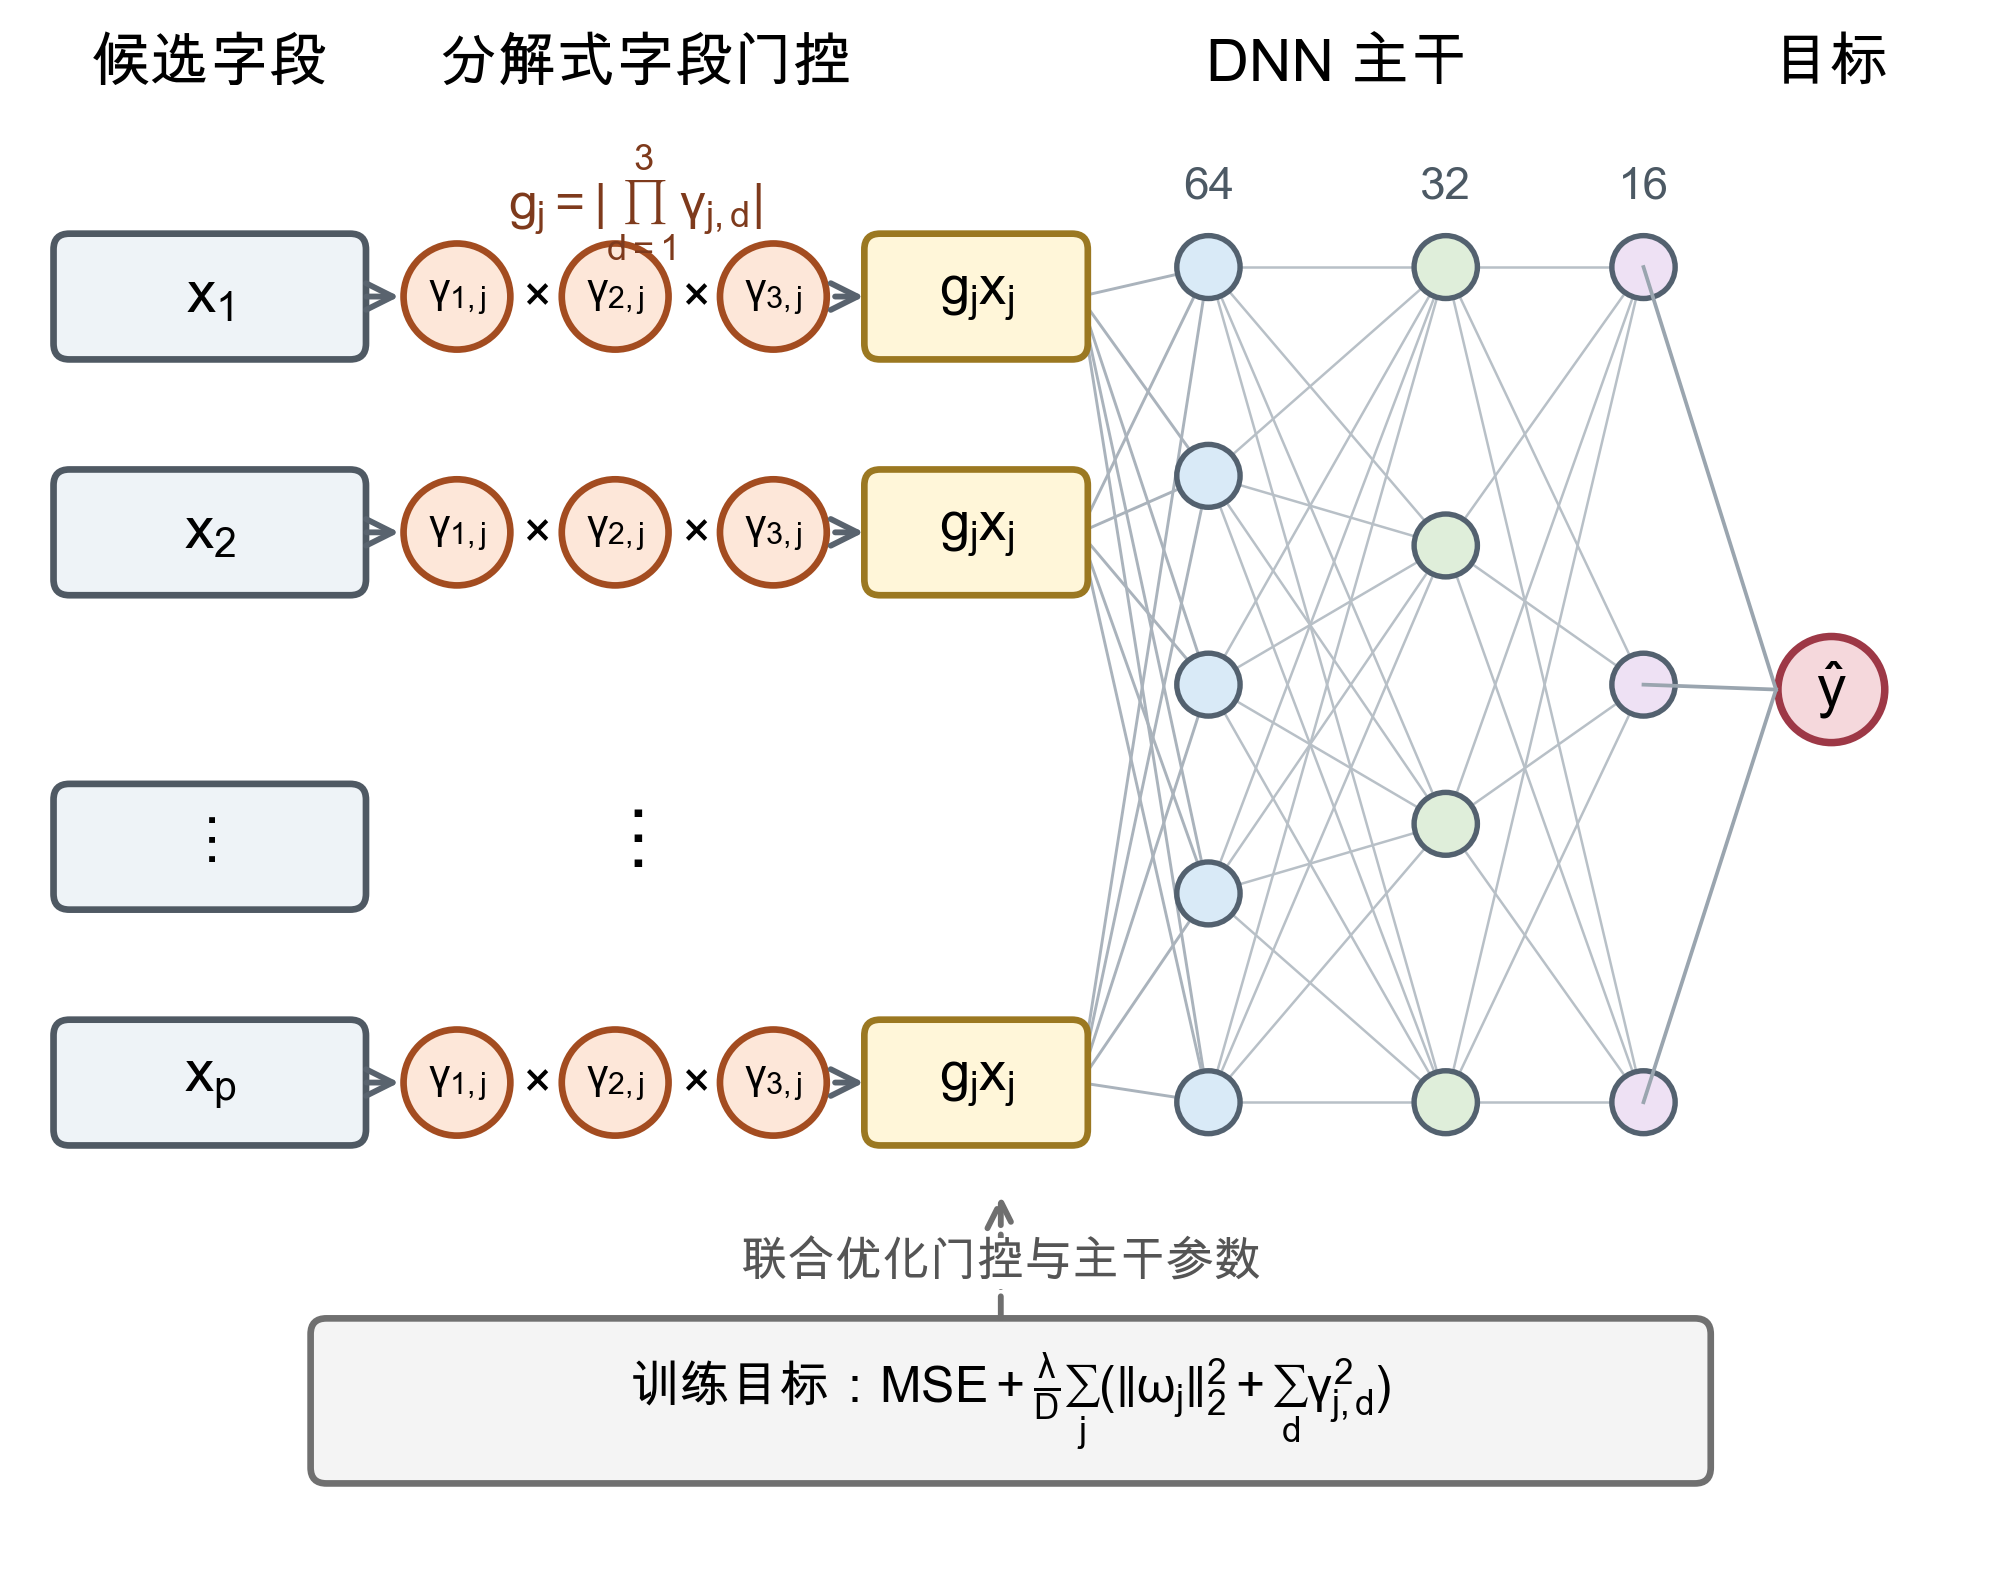
\includegraphics[width=\columnwidth]{fig_architecture.png}
\figbicaption{输入字段分解式稀疏门控网络结构}{Architecture of the input-wise factorized sparse gating network}
\label{fig:arch}
\end{figure}

训练收敛后，大量 $g_j$ 达到数值零，保留字段与淘汰字段之间形成明显间隔。正则强度 $\lambda$ 在独立校准目标的验证集上选择：在最佳验证 $R^2$ 的 0.005 容差内取最大 $\lambda$，并在全部目标上固定为 0.005。活跃阈值固定为 $\tau_g=0.01$，同时报告 $10^{-6}$ 至 $10^{-1}$ 的阈值扫描。本文不宣称完全取消阈值，而是利用门控值的断崖式分布降低结果对阈值的敏感性，避免针对每个目标人工调节。

\subsection{独立确认与审查输出}

取 $A=\{f_j\in\widetilde F:g_j\geq\tau_g\}$，在 $A$ 上重新训练一个不含门控的普通 DNN，以测试 $R^2$ 确认该字段集合本身的联合重构能力。门控模型只负责生成候选集合，论文中的最终精度均来自独立重训，避免把正则化训练过程的偏差当成字段贡献。

单个受保护目标的审查记录由三部分组成：第一类关系及牵连字段 $E_s$；第二类紧凑证据集 $A$；风险坐标 $(|A|/|\widetilde F|,\rho(s\mid A))$。在具体发布流程中，审查人员先处理规则库命中的共发布组合，再根据风险坐标确定是否需要降精度、延迟或进一步聚合；处理后的字段集合必须重新进入图~\ref{fig:flow}，而不能把一次定位结果直接当作永久阻断清单。

\section{实验与结果分析}

\subsection{数据角色与实验设置}

实验使用两个数据集，二者承担不同的论证角色，见表~\ref{tab:data}。PJM Data Miner 提供公开的市场与运行数据\cite{ref-ma-pjm,ref-pjm-dataminer}，故 PJM 实验不用于证明真实密级跨越，而用于验证方法在真实异质字段上的定位与方法比较。RTS-GMLC 是面向现代电力系统运行研究的标准算例\cite{ref-rtsgmlc}，本文基于其 2020 年负荷和新能源曲线逐小时进行交流潮流计算，以常见发布口径的系统级、区域级及分燃料汇总量为候选，以具名节点、线路和机组状态为保护目标，形成与发布审查一致的“汇总量到设备状态”方向。

\begin{table*}[!tbp]
\centering
\tabbicaption{两个数据集在实验中的角色与字段边界}{Roles and field boundaries of the two datasets}
\label{tab:data}
\zihao{6}\setlength{\tabcolsep}{4.5pt}
\begin{tabular}{p{2.1cm}p{2.0cm}p{4.7cm}p{5.4cm}}
\toprule
数据集 & 样本与候选 & 候选字段 & 目标字段及论证角色 \\
\midrule
PJM 2025 & 8760 小时；清洗后 69 个数值字段 & 负荷、发电结构、备用、价格与交换功率等公开字段 & 每次遮蔽 1 个公开字段作为目标，共 12 个；验证真实异质数据上的定位与方法比较，不作为真实密级证据 \\
RTS-GMLC & 8784 小时；58 个发布候选，去除 12 个恒定字段后可用 46 个 & 系统、区域、燃料类型汇总量及时间字段 & 从 130 个设备级状态中选 12 个，包括节点电压相角、线路负载率、具名机组出力和投入状态；验证汇总发布量对设备状态的重构风险 \\
\bottomrule
\end{tabular}
\end{table*}

主干网络含 64、32、16 个隐藏单元，激活函数为 ReLU，训练 200 轮，批大小 50，采用 Adam 优化器\cite{ref-kingma-adam}，学习率 $10^{-3}$。样本按 8:2 随机划分，随机种子固定为 42。所有方法使用相同候选池、数据划分和普通 DNN 重训流程。评价指标为测试 $R^2$、选中字段数及字段占候选比例。

\subsection{两步前置剥离结果}

规则库核对官方定义及物理与会计关系。其中，PJM 包括日前和实时电价三分量分解、净交换账目关系、分燃料出力汇总及功率平衡；RTS-GMLC 包括系统负荷与三区负荷求和、系统功率平衡、分区和分燃料发电汇总，以及具名机组或跨区线路参与相应汇总的组成关系。第二步在这些字段剥离后继续搜索高确定性替代路径。表~\ref{tab:strip} 给出 RTS-GMLC 的结果。

\begin{table}[!tbp]
\centering
\tabbicaption{RTS-GMLC 的两步前置剥离结果}{Two-step pre-localization stripping on RTS-GMLC}
\label{tab:strip}
\zihao{6}\setlength{\tabcolsep}{3.0pt}
\begin{tabular}{lcccc}
\toprule
目标类别 & 起点 & 规则库 & 路径搜索 & 剩余 \\
\midrule
节点电压相角（3 个） & 46 & 0 & 0 & 46 \\
线路负载率（5 个） & 46 & 3 & 0 & 43 \\
机组 121 核电出力 & 46 & 4 & 14 & 28 \\
其余机组量（3 个） & 46 & 4 & 0 & 42 \\
\bottomrule
\end{tabular}
\end{table}

三组目标的结果说明了两步剥离与后续定位的分工。节点电压相角未命中已知组成关系，也不存在 $R^2>0.99$ 的线性等价路径，因而其后续重构能力由隐性统计关系解释。线路负载率命中区域净送出这一规则牵连关系，但剥离后未发现新的高确定性替代路径。机组 121 的四级汇总字段全部剥离后，仍需逐层切断 14 条替代路径，说明仅维护一张公式清单不能覆盖重复口径形成的规则闭包。完成前置剥离后，普通 DNN 仍将该机组出力重构到 0.9999，表明剩余能力不是被遗漏的直接汇总字段，而是调度格局中的隐性联合关系。

\subsection{门控演化与阈值敏感性}

以 PJM 净实际交换功率为例，前置剥离后有 48 个候选字段，全量 DNN 的测试 $R^2$ 为 0.9673。图~\ref{fig:gate}(a) 展示门控演化：各字段从 1 同时出发，训练中逐渐分为稳定非零组与数值零组。最终 35 个字段的门控值为 0，13 个保持非零；阈值在 $10^{-13}$ 至 $6\times10^{-3}$ 内得到相同的 13 个非零字段。采用全局固定阈值 0.01 时得到 11 个字段，其上独立重训的测试 $R^2$ 为 0.9605，与全量模型相差 0.0068。

\begin{figure}[!tbp]
\centering

\includegraphics[width=\columnwidth]{fig_gate_evolution.png}
\figbicaption{净实际交换功率的门控演化与阈值响应}{Gate evolution and threshold response for net actual interchange}
\label{fig:gate}
\end{figure}

门控值最高的字段包括预估小时负荷、燃气出力、核电占比和燃煤出力等，符合交换功率受区域供需差额影响的业务认识。值得注意的是，预估小时负荷按六类边际相关性综合得分仅排第 40 位，却具有最高门控值；六类相关性指标与门控值的 Spearman 系数仅为 0.057。由此可见，边际相关强度与多字段联合推断中的必要性并不等价，这也是不在门控前进行强相关性裁剪的原因。

\subsection{12 个目标的定位结果}

图~\ref{fig:multi} 汇总 PJM 12 个目标的全量字段、门控选中字段和其余字段重训结果。门控平均从 46.2 个候选中保留 13.1 个，占 28.3\%；选中字段的平均测试 $R^2$ 为 0.8512，略高于全量字段的 0.8438。日前阻塞价、日前主用备用总量和净实际交换功率分别保留 20、10 和 11 个字段，测试 $R^2$ 为 0.7077、0.8544 和 0.9605，说明方法既能处理较弱的市场价格关系，也能处理较强的功率平衡关系。

\begin{figure*}[!tbp]
\centering
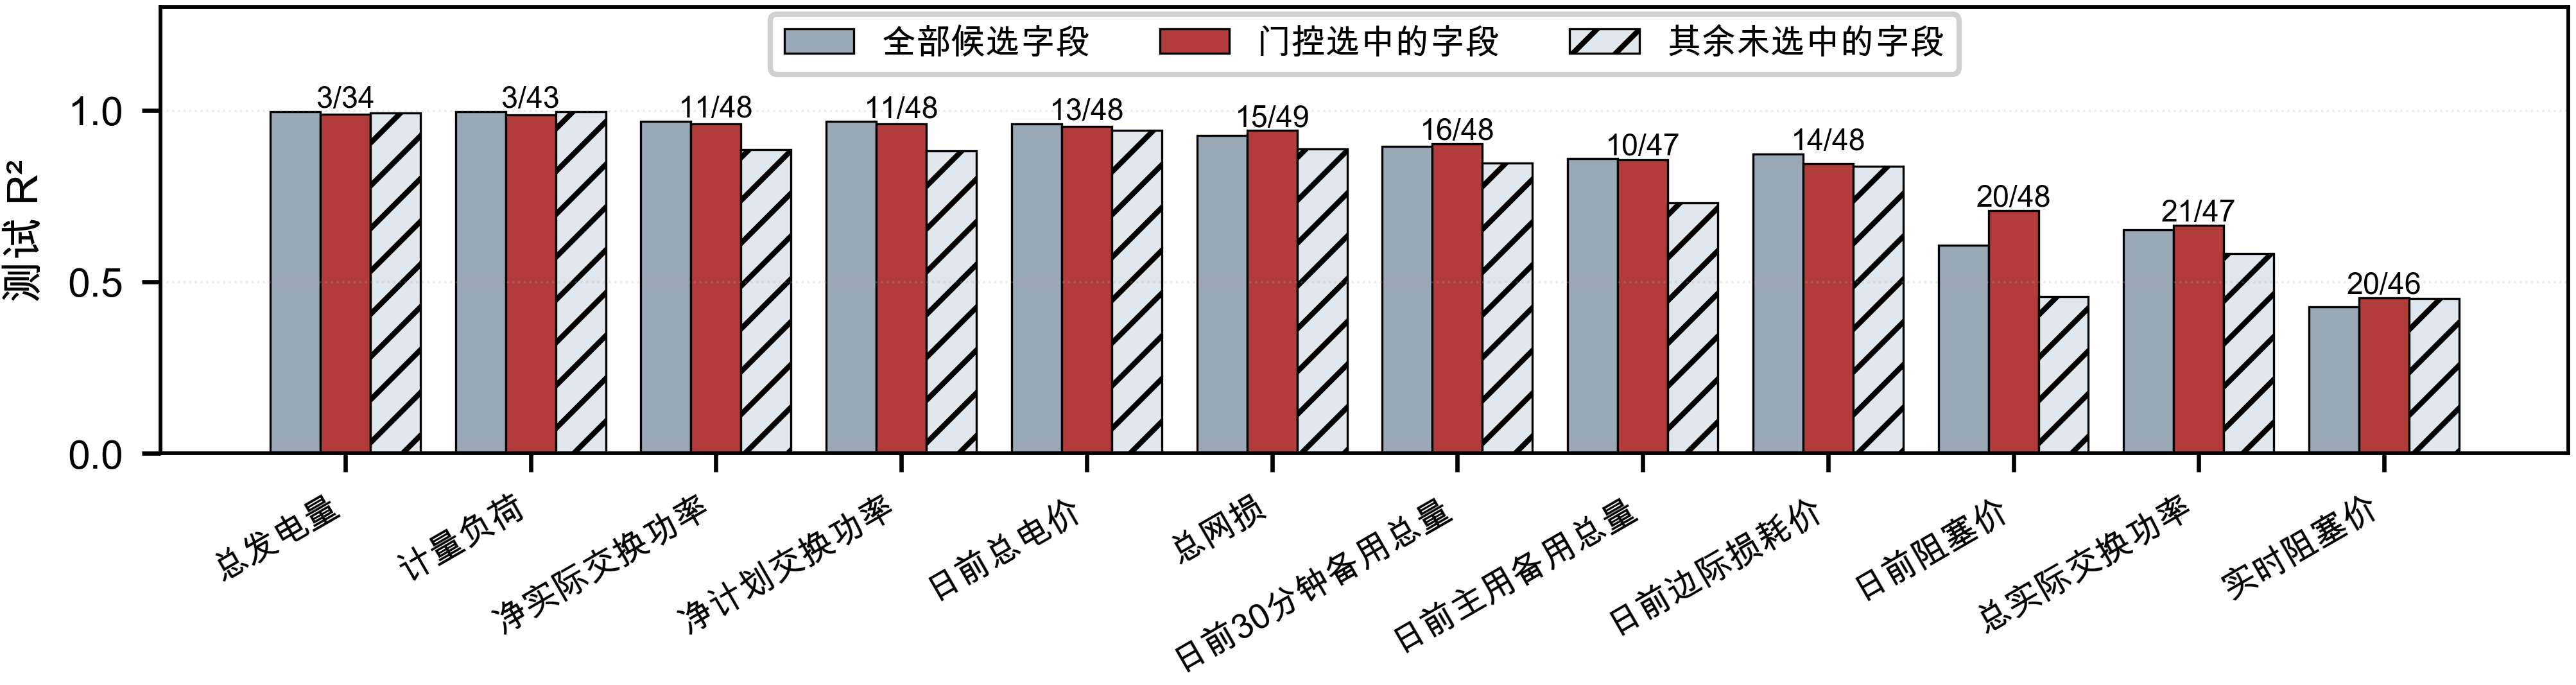
\includegraphics[width=0.89\textwidth]{fig_multitarget.png}
\figbicaption{PJM 12 个目标的推断源定位结果}{Inference-source localization results for 12 PJM targets}
\label{fig:multi}
\end{figure*}

图中其余未选中字段仍有一定重构能力，平均 $R^2$ 为 0.7905；RTS-GMLC 上由于系统、区域和燃料汇总量之间可相互替代，其余字段甚至达到 0.9745。该现象不否定式（4）的证据集定义，而说明电力数据中的推断源通常不唯一。因此，本文不把“未选中字段精度应接近零”设置为方法成立条件，也不据此宣称删除一次选中的字段即可阻断风险。

RTS-GMLC 12 个目标平均由 42.2 个候选中选出 8.0 个，占 18.9\%，选中字段平均测试 $R^2$ 为 0.9743，全量字段为 0.9837。其中 218 号联合循环机组使用 4 个汇总字段时 $R^2$ 为 0.9989，而线性回归仅为 0.8489，说明仅以线性相关或线性模型审查会显著低估非线性重构能力。

\subsection{对比实验}

选择 STG\cite{ref-stg}、LassoNet\cite{ref-lassonet}、XGBoost 和 Lasso 作为对比。主比较采用同预算协议：本文方法对每个目标确定字段数 $n$，其余方法按自身重要性排序取前 $n$ 个，再由同一普通 DNN 重训。图~\ref{fig:cmp} 给出逐目标结果。本文方法在 PJM 和 RTS-GMLC 上的平均测试 $R^2$ 分别为 0.8512 和 0.9743，均为最高；次优 STG 分别为 0.8420 和 0.9423。PJM 上各方法差距较小，RTS-GMLC 上扩大到 0.0321，说明候选字段冗余增多时，字段取舍质量的影响更明显。

\begin{figure*}[!tbp]
\centering

\includegraphics[width=0.89\textwidth]{fig_method_compare.png}
\figbicaption{同预算下各方法在两个数据集上的逐目标测试 $R^2$}{Per-target test $R^2$ under equal feature budgets}
\label{fig:cmp}
\end{figure*}

为避免同预算协议掩盖各方法自身的稀疏程度，表~\ref{tab:self} 进一步列出各方法按自身判据决定字段数的结果。PJM 上本文方法以 28\% 的字段取得最高平均精度；RTS-GMLC 上 LassoNet 和 XGBoost 的精度略高，但分别使用 98\% 和 45\% 的候选字段，本文方法以 19\% 的字段位于精度--字段数帕累托前沿的最稀疏端。因此，本文方法的结论应表述为“同字段预算下定位更准，开放预算下实现更有竞争力的稀疏--精度折中”，而非所有条件下绝对精度最高。

\begin{table*}[!tbp]
\centering
\tabbicaption{各方法自主确定字段数时的平均结果}{Average results when each method determines its own feature count}
\label{tab:self}
\zihao{6}\setlength{\tabcolsep}{5.2pt}
\begin{tabular}{lccc|ccc}
\toprule
\multirow{2}{*}{方法} & \multicolumn{3}{c|}{PJM} & \multicolumn{3}{c}{RTS-GMLC} \\
\cmidrule(lr){2-4}\cmidrule(lr){5-7}
 & 字段数 & 占比/\% & $R^2$ & 字段数 & 占比/\% & $R^2$ \\
\midrule
本文方法 & \textbf{13.1} & \textbf{28} & \textbf{0.8449} & \textbf{8.0} & \textbf{19} & 0.9748 \\
STG & 14.2 & 31 & 0.8411 & 10.7 & 25 & 0.9735 \\
LassoNet & 41.1 & 89 & 0.8439 & 41.6 & 98 & \textbf{0.9837} \\
XGBoost & 21.8 & 47 & 0.8330 & 19.1 & 45 & 0.9791 \\
Lasso & 16.4 & 36 & 0.7670 & 16.7 & 41 & 0.9387 \\
\bottomrule
\end{tabular}
\end{table*}

\subsection{发布口径变化与风险解释}

为检验发布口径本身对风险的影响，在同一组 RTS-GMLC 潮流解上设置两种候选池：v1 仅含系统级和区域级粗汇总，可用字段 24 个；v2 增加区域分燃料发电、区域发电总量和时间字段，可用字段 46 个。两种设置的目标、样本和模型完全一致。全量模型平均 $R^2$ 从 0.9633 增至 0.9837；用 $1-R^2$ 表示尚不能重构的部分，其平均值从 0.0367 降至 0.0163，即口径细化后减少 55.5\%。12 个目标中 11 个的可重构风险上升，3 个具名机组量的 $1-R^2$ 下降 99\% 以上。

这一结果给出了与方法输出直接对应的发布场景：在规则库已经剥离目标参与的系统、区域和燃料汇总后，新增的其他分区信息仍使机组组合格局更易恢复。风险来自字段组合而非某个字段名称。与此同时，风电机组目标是唯一反例，说明“口径越细必然越危险”不能作为统一发布规则，仍需对每个保护目标执行组合审查。

图~\ref{fig:risk} 以字段占比和重训 $R^2$ 表示风险集中度与强度。少量字段即可高精度恢复的目标位于左上区域，适合优先审查对应的共发布组合；需要较多字段才能恢复的目标说明风险较分散，不宜把一次定位结果直接转化为单字段禁发清单。

\begin{figure}[!tbp]
\centering

\includegraphics[width=\columnwidth]{fig_risk_map.png}
\figbicaption{受保护目标的推断风险坐标}{Inference-risk coordinates of protected targets}
\label{fig:risk}
\end{figure}

\subsection{数据降级条件下的结果}

针对实际数据的缺失与延迟，在 PJM 上选择强、中、弱三种目标，考察 6 h 块状缺失、整字段缺失和字段延迟。5 个随机种子下，净实际交换功率、日前主用备用总量和日前阻塞价的基准 $R^2$ 标准差依次为 0.0012、0.0071 和 0.0525。表~\ref{tab:rob} 给出较强降级水平下的结果。强目标在 30\% 块状缺失和 3 h 延迟时仍达到 0.9199 和 0.9516；各条件下选中子集与全量模型精度接近。弱关系波动较大，审查时应报告区间。

\begin{table}[!tbp]
\centering
\tabbicaption{较强数据降级条件下的测试 $R^2$（全量/子集）}{Test $R^2$ under severe data degradation (full/subset)}
\label{tab:rob}
\zihao{6}\setlength{\tabcolsep}{2.4pt}
\begin{tabular}{lccc}
\toprule
降级条件 & 净交换 & 主用备用 & 阻塞价 \\
\midrule
30\% 块状缺失 & 0.9199/0.9281 & 0.7710/0.7662 & 0.6681/0.7133 \\
20\% 整字段缺失 & 0.9533/0.9555 & 0.8062/0.8065 & 0.6410/0.6626 \\
3 h 数据延迟 & 0.9516/0.9404 & 0.8431/0.8771 & 0.6488/0.6265 \\
\bottomrule
\end{tabular}
\end{table}

\section{结论}

本文面向电网数据拥有方的历史数据发布前审查，研究拟发布字段组合对未发布运行状态的重构风险，并将审查对象统一划分为规则可解释关系与隐性统计关系。通过规则库闭包和高确定性替代路径搜索，在进入推断源定位前剥离第一类关系；随后将分解式结构稀疏机制作用于深度网络输入字段，并以普通网络独立重训确认紧凑风险证据集。

实验表明，PJM 12 个目标平均使用 28.3\% 的候选字段即可达到全量字段的重构能力；RTS-GMLC 中使用 18.9\% 的汇总字段可将设备级目标平均重构到 0.9743。同预算下，本文方法在两个数据集上均取得最高平均精度；开放字段预算时，方法位于稀疏--精度帕累托前沿的最稀疏端。发布口径由 24 个粗粒度字段细化到 46 个字段后，平均 $1-R^2$ 下降 55.5\%，说明逐字段密级判断不足以覆盖组合推断风险。

本文输出的是证明风险存在的一组紧凑字段证据，而非唯一推断路径或可直接执行的最小阻断集。对信息高度冗余的目标，移除一次定位出的字段后仍可能存在替代路径；因此实际处置后必须重新审查。后续工作将研究多目标共同约束下的最小代价处置，以及面向时序外推场景的跨期稳定性。

\begin{thebibliography}{99}
\zihao{6}\linespread{1.05}\selectfont
\setlength{\itemsep}{0pt}
\bibitem{ref-liu-cps}
刘涛, 田捷, 王杰, 等. 信息物理融合系统的综合安全威胁与防御研究[J]. 自动化学报, 2019, 45(1): 5-24.

LIU Tao, TIAN Jie, WANG Jie, et al. Integrated security threats and defense of cyber-physical systems[J]. Acta Automatica Sinica, 2019, 45(1): 5-24.

\bibitem{ref-ma-pjm}
马子明, 钟海旺, 李竹, 等. 美国电力市场信息披露体系及其对中国的启示[J]. 电力系统自动化, 2017, 41(24): 49-57.

MA Ziming, ZHONG Haiwang, LI Zhu, et al. Information disclosure system in American electricity market and its enlightenment for China[J]. Automation of Electric Power Systems, 2017, 41(24): 49-57.

\bibitem{ref-zhu-sharing}
邢汇笛, 龚钢军, 翟明岳, 等. 电力数据共享安全防护与隐私保护综述[J]. 综合智慧能源, 2024, 46(5): 30-40.

XING Huidi, GONG Gangjun, ZHAI Mingyue, et al. Research on security and privacy protection of electric power data sharing[J]. Integrated Intelligent Energy, 2024, 46(5): 30-40.

\bibitem{ref-liu-data-inference}
刘烃, 王子骏, 刘杨, 等. 数据推断: 信息物理融合系统数据泄露威胁范式和防御方法[J]. 中国科学: 信息科学, 2023, 53(11): 2152-2179. DOI: 10.1360/SSI-2022-0362.

LIU Ting, WANG Zijun, LIU Yang, et al. Data inference: data leakage paradigms and defense methods in cyber-physical systems[J]. Scientia Sinica Informationis, 2023, 53(11): 2152-2179. DOI: 10.1360/SSI-2022-0362.

\bibitem{ref-sankar}
Sankar L, Rajagopalan S R, Mohajer S, et al. Smart meter privacy: A theoretical framework[J]. IEEE Transactions on Smart Grid, 2013, 4(2): 837-846.

\bibitem{ref-giaconi}
Giaconi G, Gündüz D, Poor H V. Privacy-aware smart metering: Progress and challenges[J]. IEEE Signal Processing Magazine, 2018, 35(6): 59-78.

\bibitem{ref-adewole}
Adewole K S, Torra V. Privacy issues in smart grid data: From energy disaggregation to disclosure risk[C]//International Conference on Database and Expert Systems Applications. Cham: Springer, 2022: 71-84.

\bibitem{ref-zhang-sgcc}
刘家男, 翁健. 智能电网安全研究综述[J]. 信息网络安全, 2016, 16(5): 78-84.

LIU Jianan, WENG Jian. Survey on smart grid security[J]. Netinfo Security, 2016, 16(5): 78-84.

\bibitem{ref-chen-privacy}
邓晓平, 张桂青, 魏庆来, 等. 非侵入式负荷监测综述[J]. 自动化学报, 2022, 48(3): 644-663.

DENG Xiaoping, ZHANG Guiqing, WEI Qinglai, et al. A survey on the non-intrusive load monitoring[J]. Acta Automatica Sinica, 2022, 48(3): 644-663.

\bibitem{ref-lan-load}
严雪颖, 秦川, 鞠平, 等. 负荷功率模型的最优特征选择研究[J]. 电力工程技术, 2021, 40(3): 84-91.

YAN Xueying, QIN Chuan, JU Ping, et al. Optimal feature selection of load power models[J]. Electric Power Engineering Technology, 2021, 40(3): 84-91.

\bibitem{ref-jiao-pv}
Jiao X Y, Sun Y Z, Peng D, et al. Photovoltaic power abnormal data cleaning based on variance change point and correlation analysis[C]//2021 6th International Conference on Power and Renewable Energy (ICPRE). Piscataway: IEEE, 2021: 1140-1145.

\bibitem{ref-deng-load}
Deng X Y, Zhang C K, Peng H, et al. Short-term load forecasting for regional power grids based on correlation analysis and feature extraction[C]//2022 7th Asia Conference on Power and Electrical Engineering (ACPEE). Piscataway: IEEE, 2022: 1081-1085.

\bibitem{ref-szekely-dcorr}
Székely G J, Rizzo M L, Bakirov N K. Measuring and testing dependence by correlation of distances[J]. The Annals of Statistics, 2007, 35(6): 2769-2794.

\bibitem{ref-reshef-mic}
Reshef D N, Reshef Y A, Finucane H K, et al. Detecting novel associations in large data sets[J]. Science, 2011, 334(6062): 1518-1524.

\bibitem{ref-xing-micdnn}
Xing Z Y, Wang Z J, Feng J L, et al. MIC-DNN: data-driven correlation analysis framework for power data[C]//2025 40th Youth Academic Annual Conference of Chinese Association of Automation (YAC). Piscataway: IEEE, 2025: 2969-2974.

\bibitem{ref-lecun-deep}
LeCun Y, Bengio Y, Hinton G. Deep learning[J]. Nature, 2015, 521(7553): 436-444.

\bibitem{ref-goodfellow-deep}
Goodfellow I, Bengio Y, Courville A. Deep learning[M]. Cambridge: MIT Press, 2016.

\bibitem{ref-breiman-rf}
Breiman L. Random forests[J]. Machine Learning, 2001, 45(1): 5-32.

\bibitem{ref-chen-xgboost}
Chen T, Guestrin C. XGBoost: A scalable tree boosting system[C]//Proceedings of the 22nd ACM SIGKDD International Conference on Knowledge Discovery and Data Mining. New York: ACM, 2016: 785-794.

\bibitem{ref-wang-meter}
Wang Y, Chen Q, Hong T, et al. Review of smart meter data analytics: Applications, methodologies, and challenges[J]. IEEE Transactions on Smart Grid, 2019, 10(3): 3125-3148.

\bibitem{ref-tibshirani-lasso}
Tibshirani R. Regression shrinkage and selection via the lasso[J]. Journal of the Royal Statistical Society: Series B, 1996, 58(1): 267-288.

\bibitem{ref-zou-enet}
Zou H, Hastie T. Regularization and variable selection via the elastic net[J]. Journal of the Royal Statistical Society: Series B, 2005, 67(2): 301-320.

\bibitem{ref-pearson}
Pearson K. Notes on regression and inheritance in the case of two parents[J]. Proceedings of the Royal Society of London, 1895, 58: 240-242.

\bibitem{ref-spearman}
Spearman C. The proof and measurement of association between two things[J]. The American Journal of Psychology, 1904, 15(1): 72-101.

\bibitem{ref-kendall}
Kendall M G. A new measure of rank correlation[J]. Biometrika, 1938, 30(1/2): 81-93.

\bibitem{ref-cover-info}
Cover T M, Thomas J A. Elements of information theory[M]. 2nd ed. Hoboken: John Wiley \& Sons, 2006.

\bibitem{ref-gretton-hsic}
Gretton A, Bousquet O, Smola A, et al. Measuring statistical dependence with Hilbert-Schmidt norms[C]//Algorithmic Learning Theory. Berlin: Springer, 2005: 63-77.

\bibitem{ref-pjm-dataminer}
PJM Interconnection. PJM Data Miner 2[EB/OL]. [2025-05-01]. https://dataminer2.pjm.com.

\bibitem{ref-kingma-adam}
Kingma D P, Ba J. Adam: A method for stochastic optimization[C]//International Conference on Learning Representations. San Diego: ICLR, 2015.

\bibitem{ref-stg}
Yamada Y, Lindenbaum O, Negahban S, et al. Feature selection using stochastic gates[C]//Proceedings of the 37th International Conference on Machine Learning. 2020: 10648-10659.

\bibitem{ref-lassonet}
Lemhadri I, Ruan F, Abraham L, et al. LassoNet: a neural network with feature sparsity[J]. Journal of Machine Learning Research, 2021, 22(127): 1-29.

\bibitem{ref-dgating}
Kolb C, Frost L, Bischl B, et al. Differentiable sparsity via D-Gating: simple and versatile structured penalization[C]//Advances in Neural Information Processing Systems. 2025, 38. DOI: 10.52202/085713-5068.

\bibitem{ref-rtsgmlc}
Barrows C, Preston E, Staid A, et al. The IEEE reliability test system: a proposed 2019 update[J]. IEEE Transactions on Power Systems, 2020, 35(1): 119-127. DOI: 10.1109/TPWRS.2019.2925557.

\end{thebibliography}

\vspace{0.4em}
\noindent{\zihao{6}\textbf{作者简介：}郑茂然（1981--），男，高级工程师，硕士，研究方向为电力系统继电保护与安全自动控制；陶文伟（1973--），男，高级工程师，博士，主要研究方向为电力监控系统网络安全与电力系统自动化；李家璐（1986--），男，高级工程师，硕士，研究方向为电力系统运行调控与电网运行风险控制。}

\end{document}
